\documentclass[conference]{IEEEtran}

\usepackage{cite}
\usepackage{graphicx}
\usepackage{tabularx, booktabs}
\hyphenation{op-tical net-works semi-conduc-tor}

\begin{document}

\title{Performance Analysis of CNN Frameworks\\for GPUs}

\author{\IEEEauthorblockN{HeeHoon Kim}
\IEEEauthorblockA{Department of Computer Science and Engineering,\\
Seoul National University, Korea\\
Email: hydrogen@snu.ac.kr}
\and
\IEEEauthorblockN{Hyoungwook Nam}
\IEEEauthorblockA{Department of Computer Science and Engineering,\\
Seoul National University, Korea\\
Email: hwnam831@snu.ac.kr}}

\maketitle

\begin{abstract}
Convolutional neural network have been successful in visual recognition tasks.
Machine learning frameworks are using GPU deep learning libraries to efficiently implement CNNs on GPUs.
This study analyzes GPU performance characteristics of Theano, Caffe, Torch and Tensorflow via benchmarking AlexNet model on them.
The GPU utilization and framework overheads are analyzed and we suggest possible optimization methods to increase efficiency.
We also identify differences between 4 convolution algorithm kernels - GEMM, direct, FFT and Winograd convolution.
Layerwise comparison and analysis show performance characteristics of the kernels.
We suggest criterions for choosing convolution kernels and methods to create efficient CNN model on the GPU.
As scaling DNN on multi-gpu context becomes important, we compare data parallelism implementations of the frameworks.
Scalability and synchronization overheads are analyzed.
We suggest possible methods to improve multi-gpu scalability of the frameworks.
Also we provide methods to build scalable DNN model on multi-gpu context.

\end{abstract}

\IEEEpeerreviewmaketitle

\section{Introduction}

\subsection{Convolutional Neural Network}
Deep neural networks(DNN) have been very successful on various machine learning tasks such as visual recognition, speech recognition and machine translation.
\cite{}%% DNN papers
Convolutional neural network(CNN), proposed by LeCun et. al., is one of the earliest successful neural network model used for image classification tasks.
\cite{}%% lenet
CNN combined with DNN breakthroughs (e.g. ReLU activation, Dropout layer, Data augumentation) outperformed previous machine learining methods on visual recognition challenge.
\cite{}%% alexnet, googlenet, VGG
Classification accuracy of CNN models have been improving over time and recent state-of-the-art programs for visual recognition tasks uses ensembles of CNN models.
\cite{}%% ILSVRC 2016 winner
CNN models are also being applied to other machine learning tasks other than image recognition. CNN can be applied to action recognition, speech recognition, natural language processing and AI playing game of Go.
\cite{}%% one of each

\subsection{Deep learning and gpu}
The biggest advantage of applying DNN is its scalability, means that larger and deeper DNN with more input data usually results in better accuracy.
Bigger DNN requires more processing power, hence training DNN by typical computer is impractical.
Luckily, computations in neural network can easily be represented as tensor or matrix operations, which can be efficiently parallelized.
Therefore parallel processing by GPU made DNN possible to train on single machine.
Deep learning frameworks have been developed for easy and efficient implementation of DNN models, and most popular frameworks support GPU acceleration by default.
\cite{} %% Caffe, Theano, Torch, CNTK, Tensorflow
Companies and researchers have been trying to implement efficient GPU kernels to improve performance.
\cite{} %% fft-conv, fbcunn, Winograd, Cuda-convnet
The most popular one is CuDNN, a GPU deep learning library created by NVIDIA that has been adopted as GPU-backend of popular frameworks.
\cite{} %% CuDNN
Convolution with CuDNN results in up to 4x performance improvement from default GPU kernels of the frameworks.
\cite{} %% convnet-benchmark
Efficiency of deep learning on single GPU has been improved a lot, however deep learning on multiple GPU still shows poor scalability.
\cite{} %% model parallelism, distributed deep learning

\subsection{Motivation}
In this study, we analyze GPU performance characteristics of convolutional neural network on different frameworks or libraries.
We choose 4 most popular deep learning frameworks, Theano, Caffe, Torch and Tensorflow by the number of github stars.
We compare differences in performance characteristics of the frameworks and identify performance limiters of each framework.
The comparison would find out detailed pros and cons of deep learning frameworks and suggest possible improvements.
Furthermore, we take a close look into GPU kernels to analyze performance characteristics of different convolution algorithms.
Based on the analysis, we provide optimization methods to implement efficient CNN model using the GPU deep learning libraries.
Also we analyze performance characteristics of the frameworks on multi-gpu context to suggest efficient implementation method to use multiple gpus.

\section{Related work}

\subsection{Previous work}
It has been only a few years since deep learning frameworks were introduced to public.
Few attempts recently tried to benchmark and compare the performance of the frameworks.
A benchmark of CNN frameworks is publicly available on Github but it has not been updated for more than an year hence it cannot be used to compare current versions of the frameworks \cite{}.
Detailed benchmark of deep learning frameworks was published by Bahrampour et. al. but it only compares frameworks by execution time.
Hence causes for the performance difference were not identified.
Also the benchmark uses older versions of CuDNN which do not support current convolution algorithms such as fft convolution and winograd convolution.
This study, however, compares newest versions of the frameworks and provide detailed analysis down to GPU kernel level.
And also we compare them on multi-gpu context which has not been done in previous studies.


\section{Background}

\subsection{Machine learning frameworks}

\subsubsection{Theano, Torch, Caffe, Tensorflow comparison}
%TODO

\subsection{Convolution algorithms}
Several methods are used to efficiently implement convolution on GPU.
Direct convolution is the most straightforward way but needs a lot of specialized kernels to optimize for various input dimensions and corner cases.
Cuda-convnet \cite{} is the efficient direct convolution library written by Alex Krizhevsky, the author of AlexNet paper.
CuDNN however, treats convolution as matrix multiplication \cite{}.
The convolution layer of K kernels with dimension R*R and W*W input with C channels is converted to multiplication of K*CRR filter matrix and CRR*NWW data matrix.
The dimensions of matrices are very big, hence the multiplication can be parallelized using highly efficient BLAS libraries.
Converting convolution to matrix might require significant amount of memory bandwidth.
However, CuDNN computes the multiplication by tiles to hide memory latency while computing \cite{}.
This method scales well on small batch sizes and can be used on all types of convolution layers.
The complexity of both methods are basically the same.

FFT convolution uses fast Fourier transform algorithm to reduce algorithm complexity \cite{}.
FFT significantly reduces the amount of workload but requires much more memory space since filters must be padded to the dimension of inputs.
However, FFT convolution cannot be applied to convolution with stride more than 1.
Winograd convolution algorithm is based on convolution as matrix multiplication but reduces algorithm complexity using Winograd's minimal filtering algorithm.
Winograd’s minimal filtering algorithm follows the idea of Strassen’s algorithm.
For example, minimal Winograd filter of 2x3 tiling reduces number of matrix multiplication from 6 to 4 \cite{}.
However, different sized kernel needs its own minimal filtering algorithm, hence CuDNN 5.0 only supports Winograd convolution for filter size of 3x3 \cite{}.

\subsection{Multi-gpu parallelism}
Multi-gpu implementation of deep neural networks can be implemented by data parallelism or model parallelism \cite{}.
On data parallelism, a batch of inputs is divided and distributed among devices.
After backpropagation, the entire gradients of network parameters must be passed to single device in order to compute stochastic gradient descent.
And then the updated parameters are distributed among devices.
Hence, the communication cost of data parallelism depends on number of parameters in the network.
AlexNet has 65M parameters, thus each iteration needs to transfer approximately 520MB of data per GPU.
On the other hand, model parallelism divides and distributes the network.
Carefully designed model parallelism of convolution layer outperforms the data parallelism \cite{}.
However, multi-gpu support on Caffe is limited to data parallelism, therefore we only compare data parallelism efficiencies of the frameworks.
Tensorflow and Torch supports both data and model parallelism while Theano doesn’t support multi-gpu natively.

\section{Experiment setup}

\subsection{System setup}
We test the frameworks on the CentOS 7.2 server with 4 octa-core Xeon-E5 cpus and 4 GTX TITAN X(GM200) gpus.
We use Cuda 7.5 and CuDNN R5 which is the latest stable release of Cuda and CuDNN.
All deep learning frameworks are updated to latest stable release on June 2016.
The versions of the frameworks fully support CuDNN R5.
Only Torch supports the latest version of Cuda-convnet3.
The detailed system environments are represented on Table \ref{} and \ref{}.

CentOS 7.2.1511 / Linux 3.10.0-327 / Inte Xeon E5-2650@2.0GHz / 128GB DDR3@1600MHz / CuDNN 5005 / Cuda 7.5 / Torch 7 ccn2.torch, cudnn.torch R5 / Theano 0.8.2 / Caffe * / Tensorflow *
%TODO

\subsection{AlexNet model}
AlexNet \cite{} is one of the earliest successful deep neural networks on image recognition task using ImageNet dataset \cite{}.
AlexNet uses 5 convolution layers to extract features and 3 fully connected layers for classification.
Each layer has rectified linear unit(ReLU) layer for nonlinear activation.
AlexNet has been frequently used for benchmarking performance of machine learning libraries, because it utilizes most of the current DNN components such as convolution, max-pooling and dropout \cite{}.
The original AlexNet model includes Local response normalization(LRN) layer, but we exclude it for benchmarking task since LRN is very rarely used in current convolutional neural networks.
The detailed layer structure of AlexNet model on this study is presented in Table \ref{}.


\begin{table*}[]
\centering
\caption{Alexnet model used on benchmarking}
\label{alex_model}
\begin{tabular}{llllllll}
Name    & Kernel(R) & Input Channels(C) & Ouput Channels(K) & Stride(K) & Sample width(W) & Params & Flop \\
Input   &           & 3                 &                   &           & 227 x 227       &        &      \\
Conv1   & 11 x 11   & 3                 & 96                & 4         & 55 x 55         & 35K    & 55G  \\
Pool    & 3 x 3     &                   &                   & 2         &                 &        &      \\
Conv2   & 5 x 5     & 96                & 256               & 1         & 27 x 27         & 614K   & 227G \\
Pool    & 3 x 3     &                   &                   & 2         &                 &        &      \\
Conv3   & 3 x 3     & 256               & 384               & 1         & 13 x 13         & 885K   & 65G  \\
Conv4   & 3 x 3     & 384               & 384               & 1         & 13 x 13         & 1.3M   & 98G  \\
Conv5   & 3 x 3     & 384               & 256               & 1         & 13 x 13         & 885K   & 65G  \\
Pool    & 3 x 3     &                   &                   & 2         &                 &        &      \\
FC6     &           & 256 x 6 x 6       & 4096              &           &                 & 37M    & 74M  \\
FC7     &           & 4096              & 4096              &           &                 & 16M    & 32M  \\
FC8     &           & 4096              & 1000              &           &                 & 4M     & 8M   \\
Softmax &           & 1000              & 1000              &           &                 &        &     
\end{tabular}
\end{table*}


\section{Results/Analysis}

\subsection{Single GPU analysis}


\subsection{characterization of different convolution algorithms}
Since forward and backward propagation of convolution layers takes most of the running time, we run the same model on different convolution kernel to characterize the performance of each convolution algorithm.
Three types of convolutions are computed for each iteration.
forward convolution(FWD) computes the layer output, backward data convolution(BD) computes backward gradient input and backward filter convolution(BW) computes gradients of network parameters.
CuDNN R5 supports matrix multiplication convolution(gemm), FFT convolution, and winograd convolution.
CuDNN has various gemm convolution algorithms and the tested algorithm is implicit gemm precomp algorithm.
Winograd convolution cannot be applied to BW convolution on CuDNN 5.0 hence we use fft convolution instead.(CuDNN 5.1RC supports winograd nonfused option)
Since the first convolution layer has stride of 4, Winograd and FFT convolution cannot be applied.
Direct convolution is tested by Torch binding of Cuda-convnet3.
All comparisons are done on Torch 7 because Torch can specify convolution algorithm on each layer and newest version of Cuda-convnet3 is only supported by Torch7.

Randomly generated batch inputs are used to remove IO latency.
The forward and backward propagation time is measured as average of 100 iterations.
The compute times and statistics of kernels are measured by NVIDIA nvprof profiler.
The theoretical floating point operation counts are calculated as 2 * K*CRR*NWW since each calculation uses 1 addition and 1 multiplication.
We compare them to actual floating-point operation counts of the kernels.
Flops of the kernels are calculated as Flop count/execution time.
FFT convolution consists of 2 FFTs and 1 complex matrix multiplication, thus statistics of those 3 kernels are added together.

\begin{figure}
  \centering
  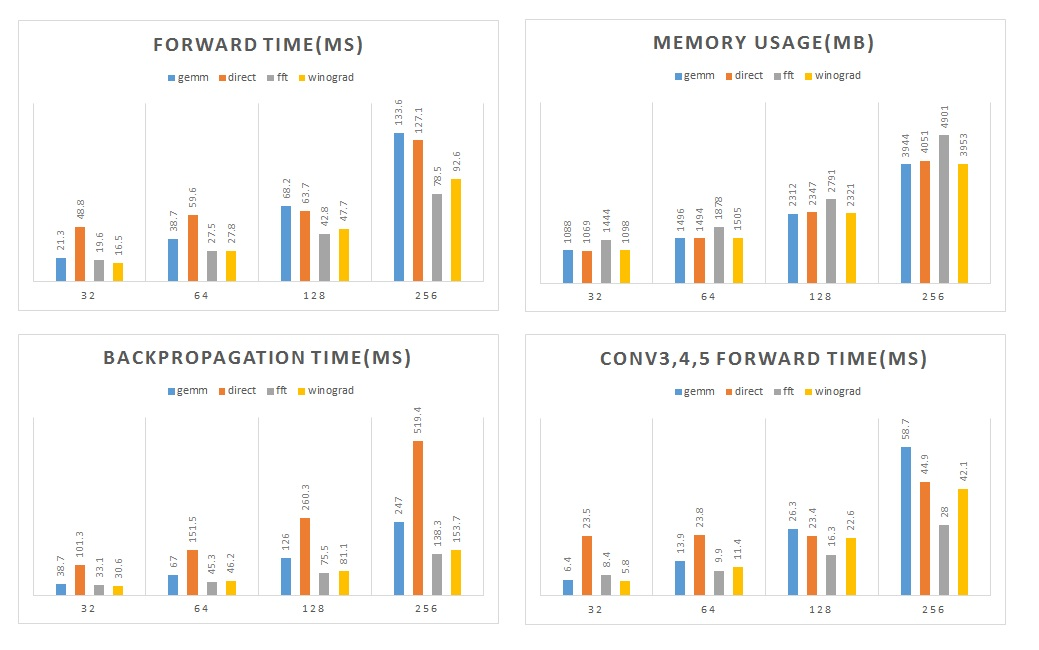
\includegraphics[width=\linewidth]{./figures/conv_time}
  \caption{Forward propagation and Backpropagation times of convolution algorithms. The times are measured as average of 100 batch iterations. 
Direct convolution is tested with cuda-convnet3 and other 3 are kernels of CuDNN R5. }
  \label{fig_conv_time}
\end{figure}

FIg \ref{fig_conv_time} shows execution time comparisons between convolution kernels.
Winograd convolution and FFT convolution always perform better than direct or gemm convolution, due to smaller floating point operations required.
FFT has smallest operations count, makes it fastest among algorithms on big batch inputs.
However FFT scales bad on smaller batch sizes because it executes 5 kernels per each layer.
The forward propagation speed comparison on conv layer 3,4,5 on (f) of Fig \ref{fig_conv_time} clearly shows the differences.
Cuda-convnet scales bad when the batch size is smaller than 128 while GEMM convolutoin sclaes almost linearly.
Winograd performs better when the batch size is smaller than 64, where theoretical operations per each layer is around 20G operations.
Winograd kernels are more efficient when the sample width is even.
When we increase the sample width of conv layer 3,4,5 from 13 to 14, the execution time of Winograd kernels decrease by 10\%.

Number of floating point operations needed for forward propagation and backward propagation kernels are equal on the same layer.
Therefore, execution time of forward and backward propagation kernels are almost symmetric on most convolution algorithms.
However, backpropagation kernels of direct convolution takes more execution time than their forward counterparts.
Especially backward filter convolution on first convolution layer takes 200ms to execute, occupying 40\% of total training time.
The reason for the slow execution is low parallelism of kernels.
The backward direct convolution kernels have small thread numbers compared to other algorithms, generating 6 times smaller thread grid size.
The backward filter convolution for the first layer generates only 1024 threads, while Titan X has 3072 CUDA cores.





\begin{figure}
  \centering
  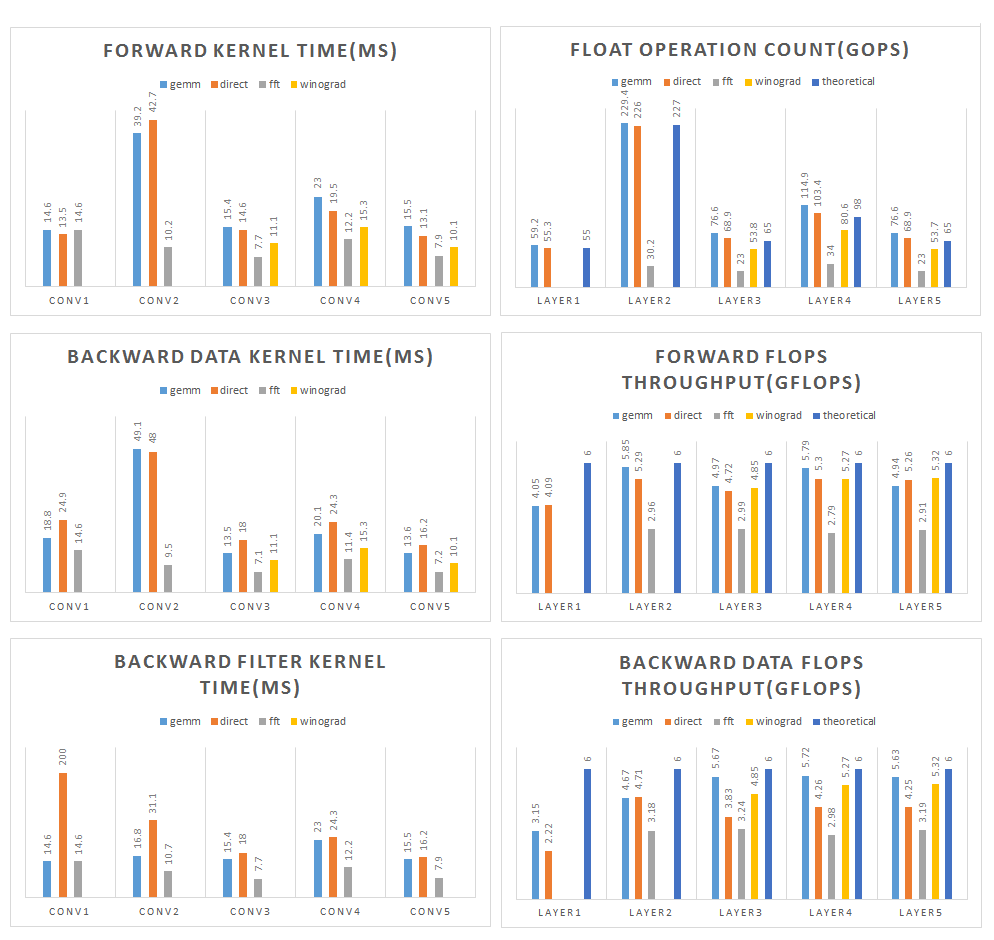
\includegraphics[width=\linewidth]{./figures/layerwise_bench}
  \caption{Layerwise analysis of convolution kernels}
  \label{fig_layerwise}
\end{figure}


\subsection{Multi GPU analysis}

\begin{itemize}
  \item Support
  \item Scalability : proportion of data exchange
  \item Synchronization cost
\end{itemize}

\section{Discussion / Conclusion}

\begin{itemize}
  \item Summary of results
  \item Compare frameworks : Implementation difference
  \item Locate bottleneck / suggest possible optimization
  \item Limitation, future research
\end{itemize}

\section*{Acknowledgment}

The authors would like to thank...

\begin{thebibliography}{1}

\bibitem{IEEEhowto:kopka}
H.~Kopka and P.~W. Daly, \emph{A Guide to \LaTeX}, 3rd~ed.\hskip 1em plus
  0.5em minus 0.4em\relax Harlow, England: Addison-Wesley, 1999.

\end{thebibliography}

\end{document}
